% Equation with label on the right side
\begin{equ}[!ht]
  \begin{equation}
    (\forall u,v \in r)(u[X]=v[X] \implies u[Y]=v[Y])
  \end{equation}
  \caption{\label{eq:gull}}
\end{equ}

% Figure
\begin{figure}
    \centering
    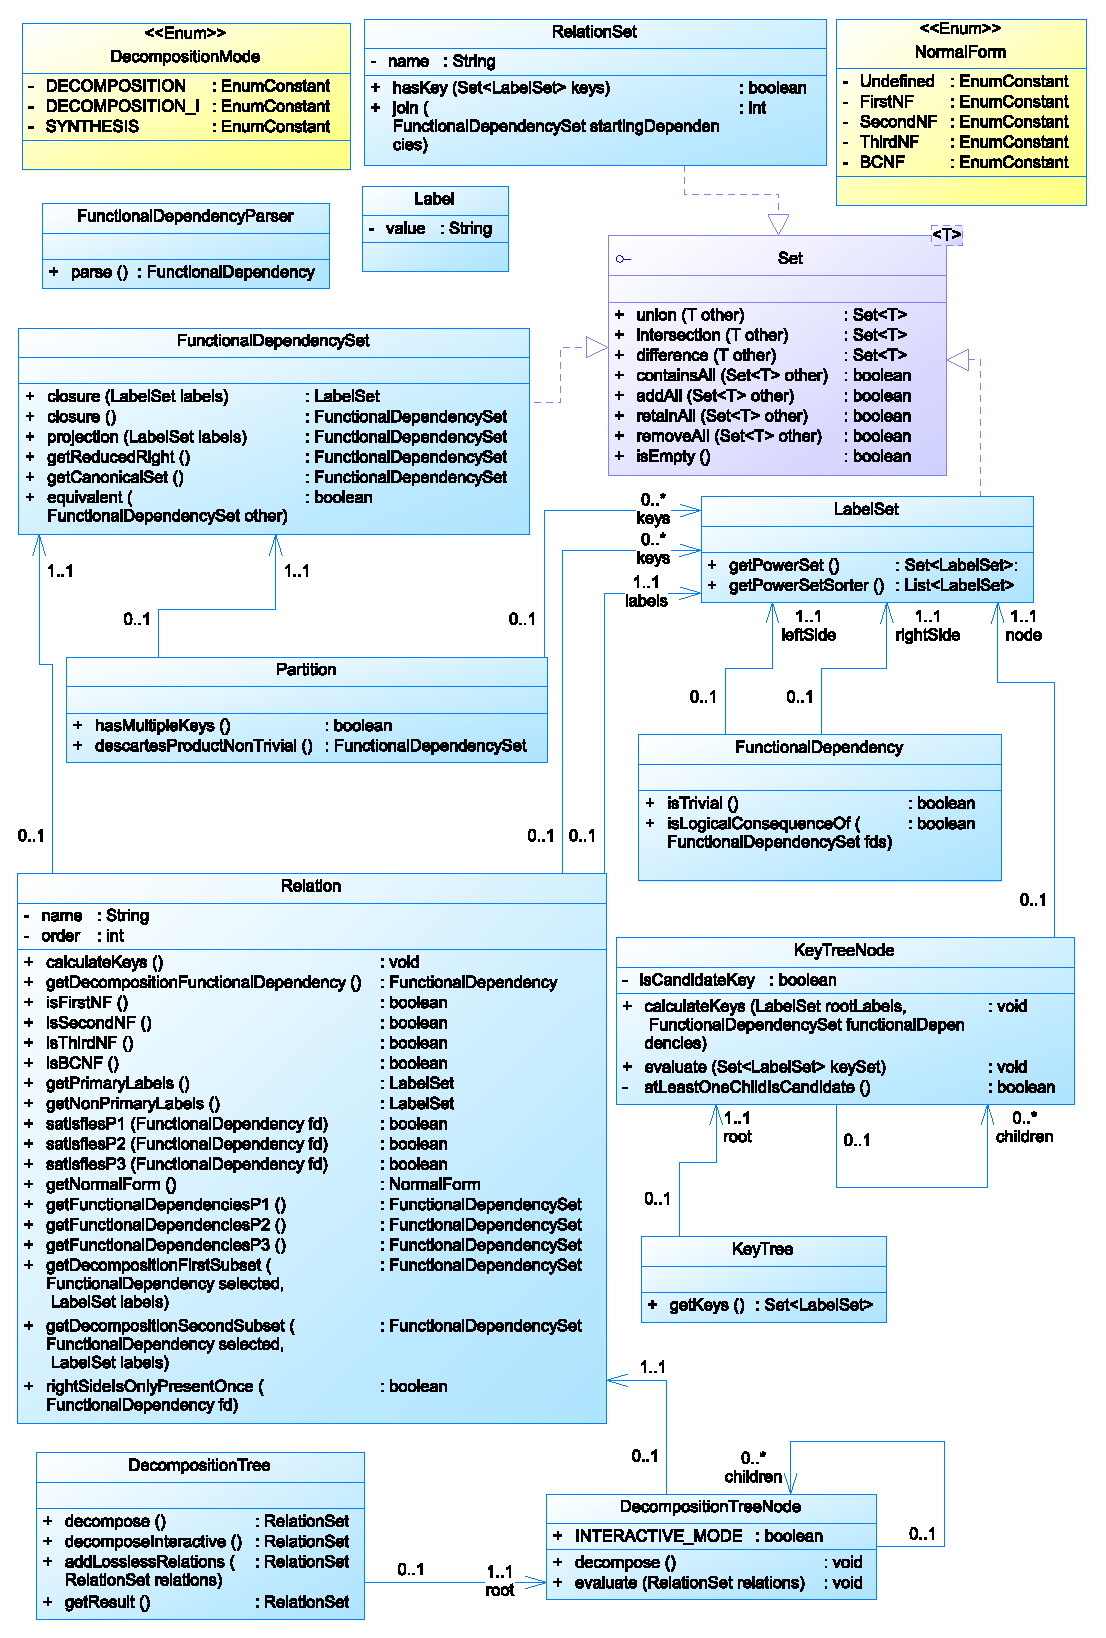
\includegraphics[width=1\textwidth]{ClassDiagram_1}
    \caption{Caption}
    \label{fig:my_label}
\end{figure}

% Code/algorithm
\linespread{1}
\begin{lstlisting}[language=Java]
import numpy as np
    
def incmatrix(genl1,genl2):
    m = len(genl1)
    n = len(genl2)
    M = None #to become the incidence matrix
    VT = np.zeros((n*m,1), int)  #dummy variable
    
    #compute the bitwise xor matrix
    M1 = bitxormatrix(genl1)
    M2 = np.triu(bitxormatrix(genl2),1) 

    for i in range(m-1):
        for j in range(i+1, m):
            [r,c] = np.where(M2 == M1[i,j])
            for k in range(len(r)):
                VT[(i)*n + r[k]] = 1;
                VT[(i)*n + c[k]] = 1;
                VT[(j)*n + r[k]] = 1;
                VT[(j)*n + c[k]] = 1;
                
                if M is None:
                    M = np.copy(VT)
                else:
                    M = np.concatenate((M, VT), 1)
                
                VT = np.zeros((n*m,1), int)
    
    return M
\end{lstlisting}

% Table